\begin{flushright}
\small{
\textit{
``Many historical and modernized systems of building with unstabilized earth exist around the globe, and comprise the housing for a large percentage of humanity. In many cases, multiple examples can be found of extant structures with many centuries of useful service life, none of which have been designed by engineers. The durability, utility, and appeal of earthen construction is thus established, and historical systems in particular express designs generally well adapted to local climate and conditions."}} \\ --- ASTM International. \\ \textit{Standard Guide for Design of Earthen Wall Building Systems : Appendix X1 : Empirical Design and Minimum Detailing Requirements for Earthen Structures}. 2010.
\end{flushright}

A side effect of rammed-earth's relative dormancy in the U.S. is a lack of centralized, homogenized research data (when compared to concrete or steel, for instance) or a unified science for guiding rammed-earth construction from wild soil to building performance and eventual deterioration. Historically, the rammed-earth building process has been guided by the immediate intuition and somatosensory judgements of experienced builders \cite{RAMMEDEARTHHOUSE}. In contemporary rammed-earth building, the scientific viewport is of great importance. Essential considerations range from the seismic behavior of geographic regions to the chemical behavior of clay particles.

Both of these construction logistics are evidenced across an array of modern building guides, codes and standards. In the empirical sense, formal guides such as ASTM E2392/E2392M (Appendix X1) appear to be relatively liberal with the techniques and quantities involved in rammed-earth construction. Granted a single-story building in a seismically low-risk area, methods such as the ``Ball Test" and the ``Roll Test" provide approximate values for design and construction. In the modern scientio-industrial sense, codes such as the New Mexico Earthen Building Materials Code demand stabilization on the order of six percent by weight of Portland cement and laboratory testing on a set of samples prepared from the site\footnote{\url{https://archive.is/2wkiN}}. Joe Dahmen (principal investigator/designer for the rammed-earth wall at M.I.T.) reported, in discussion with a Tuscon-based rammed-earth builder, ``builders often increase the amount of Portland cement to double the amount specified to avoid a shortage of cement in the mix, which is measured by approximate means in the field.\footnote{\url{https://archive.li/WP2Uf}}"

The constitutional complexity of rammed-earth is a challenge and an opportunity. It is a challenge because the emergent performance of a rammed-earth is determined by an ensemble of microscopic particles and resultant pore structure, fuzzy pre-factors of construction such as water content, compaction energy, the configuration of the structure, local topology, hydrology, and weather/climate patters, to name only a few factors.

This complexity may also be one of rammed-earth's great assets. By keeping track of a finite representation of these parameters in a centralized, visible, and open format, an outward-facing standard may evolve not simply around ensuring an arbitrary value of mechanical strength, but also around the customization of performance per local geology and geography.

This is a case for empirical science in rammed-earth building and standardization, mainly but not exclusively opposed to analytical models and ``top-down" standards which lack the capability to express this complexity without years of abstracting laboratory research and much mathematical rigidity. Whether empirical data is somehow integrated or plainly recorded and made accessible, it is a quick and transparent mode of science that has the potential to become more detailed and also adapting in time with new data. The artistic aspect of rammed-earth has not prohibited experimentation with tempers such as lime, straw, or chaff \cite{RAMMEDEARTHHOUSE}. An empirically open standard is able to facilitate and propagate new practices, while a closed, prescribed standard prohibits timely adaptability.

A notable link between the geographic and the geological is the steady accumulation of pedological information over time. Saliently, the U.S. Soil Survey began in 1899 as an endeavor based in the utility of knowledge about soil for e.g. agricultural and constructional purposes. Since, the database has been digitized and covers more than ninety-five percent of the nation's counties \footnote{\url{http://archive.li/hD4CZ}}. Of note is SoilGrids\footnote{\url{http://archive.is/l07N3}}, a machine learning-based pedological model drawing from several independent sources and projecting results at a spatial resolution of 250 meters.

Queryable soil properties of the Soil Survey include: percent clay, percent sand, percent silt, linear extensibility, plasticity index, AASHTO group classification, and Unified soil classification.

\begin{figure}[H]
  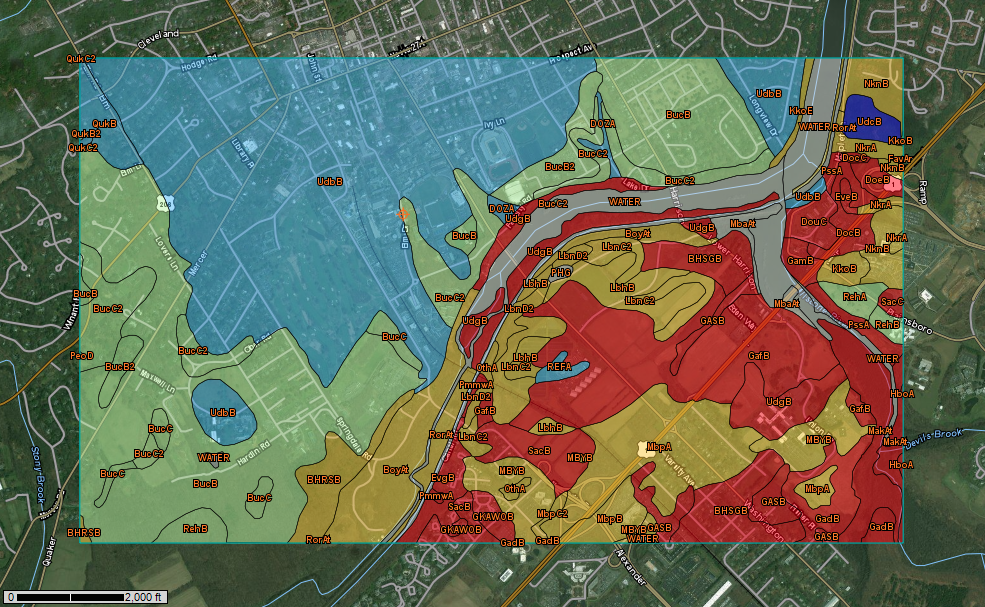
\includegraphics[scale=0.45]{wss1}

  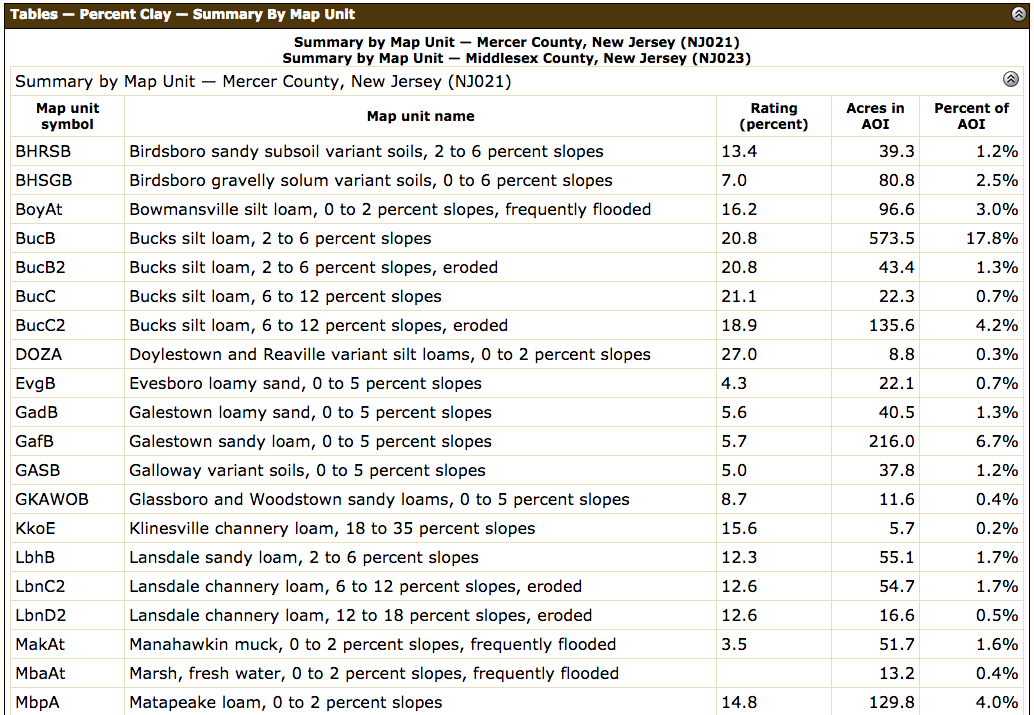
\includegraphics[scale=0.43]{wss2}
\end{figure}






\begin{flushright}
\small{
\textit{``What holds for the pyramids and the ant hills holds for all our logistics and manufacturing operations."}}
\end{flushright}

\vspace{5mm}

\begin{flushright}
\small{
\textit{``The pyramid and the quarry grow at the same time. If the pyramid is a positive architecture (y $<$ 0), the quarry is its negative. Such positive-negative pairs are everywhere in history and geography, even though modern advances in transportation technology tend to obscure them" }}\\ --- Adrian Bejan \\ \textit{Advanced Engineering Thermodynamics, Third Edition}. 2006.
\end{flushright}

A main consequence of readily available geo-spatial information is the optimization of soil convergence as an area-to-point flow. Adrian Bejan describes this phenomenon in pyramid and ant hill construction, wherein the location and the shape of pyramids and ant hills around the world are predicted by applying a principle of least work \cite{FLOWFOSSIL}.

Saliently, this connection between ancient principle and modern technology stands to offer a previously unseen level of accountability for rammed-earth building. Designers are able to openly access (Web Soil Survey:SQL, SoilGrids:JSON) soil information local to their site, determine where and not where soil may be accessed, and predicate rammed-earth material composition around the local soilscape and climate. Emergy-oriented design decisions can be made between, for instance, adding two percent more cement, or transporting additional clay from twenty miles away.
